\section{Algorithme approch\'e sur des graphes}

Soit \textit{G} un graphe tel qu'il n'existe qu'une seule feuille. Par
cons\'equent chaque noeud ne poss\`ede qu'un seul et unique fils. Nous
prendrons un arbre de ce type mais de taille 3.

Si nous appliquons l'algorithme vu en cours nous obtiendrons une
couverture optimale, et si nous appliquons notre algorithme nous
obtiendrons une couverture deux fois plus grande que la couverture optimale.


\bigskip


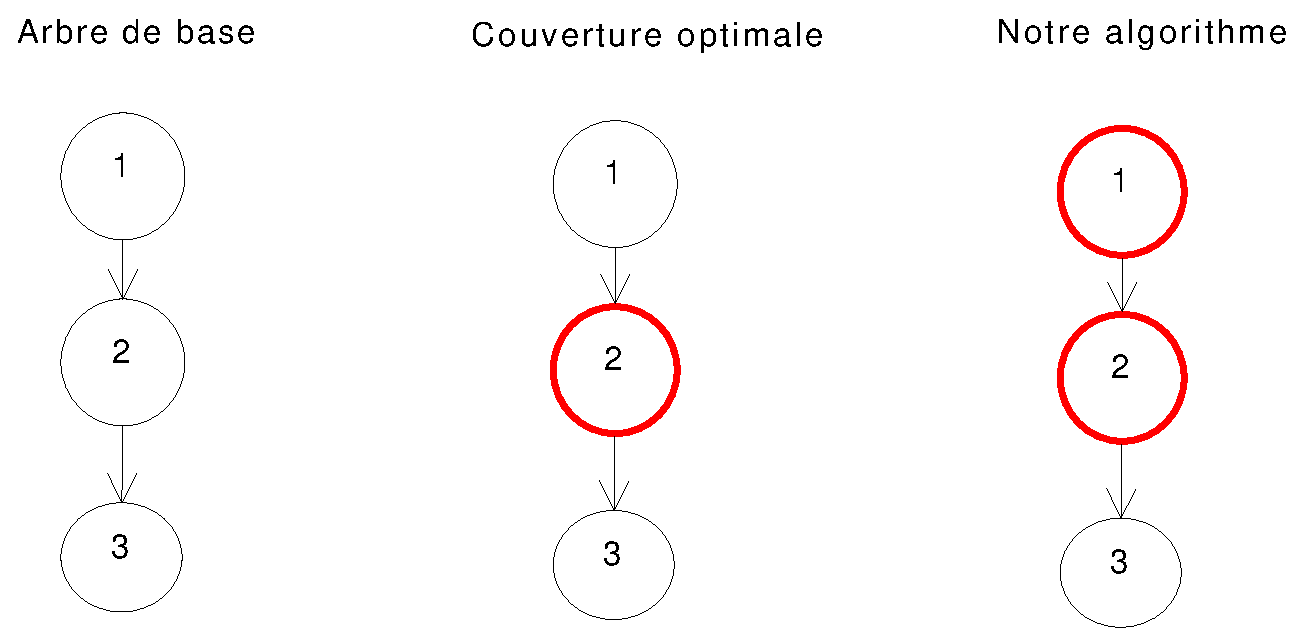
\includegraphics[width=15cm]{arbredoublecouverture}

On constate que nous prenons les noeuds 1 et 2, alors que l'algorithme
de couverture optimale ne prend que le noeud 2. Nous avons donc 2 fois
plus de noeuds dans notre couverture que l'algorithme optimale, c'est
donc une couverture 2 approch\'e.
